\newif\ifen
\newif\ifes
\newcommand{\en}[1]{\ifen#1\fi}
\newcommand{\es}[1]{\ifes#1\fi}
\entrue
\documentclass[a0,portrait]{a0poster} %A0 841mm x 1189mm
\usepackage{multicol} % This is so we can have multiple columns 
\columnsep=80pt % This is the amount of white space between the columns in the poster
\columnseprule=3pt % This is the thickness of the black line between the columns in the poster

\usepackage[svgnames]{xcolor} % Specify colors by their 'svgnames', for a full list of all colors available see here: http://www.latextemplates.com/svgnames-colors
\usepackage[makeroom]{cancel} % \cancel{} \bcancel{} etc
\usepackage{multirow}
%\usepackage{times} % Use the times font
%\usepackage{palatino} % Uncomment to use the Palatino font
%\usepackage[sfdefault]{AlegreyaSans}
\usepackage[sfdefault]{AlegreyaSans}

\usepackage{graphicx} % Required for including images
\graphicspath{{figures/}} % Location of the graphics files
\usepackage{booktabs} % Top and bottom rules for table
\usepackage[labelfont=bf]{caption} % Required for specifying captions to tables and figures
\captionsetup[subfigure]{font=Large}
\captionsetup[figure]{font=Large}
\usepackage{amsfonts, amsmath, amsthm, amssymb} % For math fonts, symbols and environments
\usepackage{wrapfig} % Allows wrapping text around tables and figures
\usepackage{bm}
\usepackage{ragged2e}
\usepackage{float} % para que los gr\'aficos se queden en su lugar con [H]
\usepackage[subrefformat=parens]{subcaption} % para \begin{subfigure}
\usepackage{tikz} % Para graficar, por ejemplo bayes networks
\usepackage{framed}
\usepackage{mdframed}
\usepackage[utf8]{inputenc}
  
\usepackage[absolute,overlay]{textpos} 
\setlength{\TPHorizModule}{1cm} %
\setlength{\TPVertModule}{1cm}	%

\newcommand{\E}{\en{S}\es{E}}
\newcommand{\A}{\en{E}\es{A}}
\newcommand{\Ee}{\en{s}\es{e}}
\newcommand{\Aa}{\en{e}\es{a}}


\usetikzlibrary{bayesnet} % Para que ande se necesita copiar el archivo  tikzlibrarybayesnet.code.tex en la misma carpeta


\newcommand{\vm}[1]{\mathbf{#1}}
\newcommand{\N}{\mathcal{N}}
\newcommand\hfrac[2]{\genfrac{}{}{0pt}{}{#1}{#2}} %\frac{}{} sin la linea del medio

% \usepackage{xr}
% \externaldocument{supplementary}
\setlength{\columnseprule}{0pt}


\addtolength{\textwidth}{40pt}
\addtolength{\oddsidemargin}{-40pt}
 
\begin{document}
% 
% \begin{textblock}{100}(18,23.25)
%  \includegraphics[width=0.1\textwidth]{auxliar/images/dc_color.pdf} 
%  \end{textblock}
% \begin{textblock}{100}(30,24)
%  \includegraphics[width=0.1\textwidth]{auxliar/images/icc-logo.jpg} 
%  \end{textblock}
%  \begin{textblock}{100}(49,24)
%  \includegraphics[width=0.1\textwidth]{auxliar/images/logo_licar.pdf} 
%  \end{textblock}
%   \begin{textblock}{100}(61,24)
%  \includegraphics[width=0.1\textwidth]{auxliar/images/logo_version_02.pdf} 
%  \end{textblock}
%  
%----------------------------------------------------------------------------------------
%	POSTER HEADER 
%----------------------------------------------------------------------------------------

% The header is divided into two boxes:
% The first is 75% wide and houses the title, subtitle, names, university/organization and contact information
% The second is 25% wide and houses a logo for your university/organization or a photo of you
% The widths of these boxes can be easily edited to accommodate your content as you see fit
\centering \fontsize{90}{90} \textbf{Bayesian inference: learning and  evolution} \\[0.5cm]  % Title
\LARGE \textbf{Gustavo Landfried}  \ \ \  \texttt{glandfried@dc.uba.ar} \\
\large 1. Universidad de Buenos Aires. Facultad de Ciencias Exactas y Naturales. Departamento de Computaci\'on. Buenos Aires, Argentina \\ 
\large 2. CONICET-Universidad de Buenos Aires. Instituto de Investigaci\'on en Ciencias de la Computaci\'on (ICC). Buenos Aires, Argentina \\


\vspace{0cm}

%\begin{paracol}{2}
\begin{multicols}{2}
% This is how many columns your poster will be broken into, a portrait poster is generally split into 2 columns
\fontsize{40}{50}\selectfont






















\centering

\texttt{github.com/glandfried/TrueSkillThroughTime}

{\fontsize{60}{72}\selectfont \textbf{TrueSkill Through Time (TTT)} \\[0.2cm]
\LARGE \textbf{Reliable initial skill estimates and historical comparability} } \\[0.8cm]

\justify 


\en{The TTT model is the current state-of-the-art skill estimator in the video game industry: it provides reliable estimates of initial skill and guarantees historical comparability. }%
\es{El modelo TTT es el estimador de habilidad actualmente estado-del-arte en la industria del video juego: ofrece estimaciones fiables de la habilidad inicial y garantiza la comparabilidad histórica. }%
%\en{Unlike the most commonly used skill estimators in the video game industry (Elo, TrueSkill, Glicko), the TTT model obtains reliable initial skill estimates and guarantees historical comparability by propagating the whole information in a single Bayesian network. }%
%\es{A diferencia de los estimadores de habilidad más utilizados en la industria del video juego (e.g Elo, TrueSkill, Glicko), el modelo TTT obtiene estimaciones fiables de la habilidad inicial y garantiza la comparabilidad histórica gracias a que propaga toda la información histórica en una única red bayesiana. }%
%
\en{Published more than a decade ago, it was not available in the programming languages with the largest scientific communities. }%
\es{Publicado hace más una década, no estaba disponible en los lenguajes de programación con mayores comunidades científicas. }%
%
\en{In this paper we offer the first package for \texttt{Julia}, \texttt{Python} and \texttt{R}, an efficient algorithm that allows millions of observations to be analyzed using any low-end CPU. }%
\es{En este artículo ofrecemos el primer paquete para \texttt{Julia}, \texttt{Python} y \texttt{R}, un algoritmo de alto desempeño que permite analizar millones de observaciones usando cualquier ordenador de gama baja. }
%

\vspace{1cm}

\textbf{Introduc\en{tion}\es{ción}.} 
\en{All skill estimators made pairwise comparisons. }%
\es{Todos los estimadores de habilidad ampliamente usados se basan en comparaciones por pares. }%
\begin{figure}[H]
\begin{subfigure}[b]{0.39\linewidth}
  \centering
  \scalebox{1.5}{
   \tikz{         
    \node[det, fill=black!10] (r) {$r$} ; 
    \node[const, below=of r, yshift=-1.5cm] (ir) {} ; 
    \node[const, right=of r] (dr) {$ r = (d > 0)$}; 
    \node[const, below=of dr, xshift=-.1cm] (r_name) {\small \en{Result}\es{Resultado}}; 
    

    \node[latent, above=of r, yshift=-1cm] (d) {$d$} ; %
    \node[const, right=of d] (dd) {$ d = p_i-p_j$}; 
    \node[const, below=of dd, xshift=-.1cm] (d_name) {\small \en{Difference}\es{Diferencia}};
    
    \node[latent, above=of d, xshift=-1.5cm, yshift=-1cm] (p1) {$p_i$} ; %
    \node[latent, above=of d, xshift=1.5cm, yshift=-1cm] (p2) {$p_j$} ; %
    

    \node[accion, above=of p1,yshift=0.5cm] (s1) {} ; %
    \node[const, right=of s1] (ds1) {$s_i$};
    \node[accion, above=of p2,yshift=0.5cm] (s2) {} ; %
    \node[const, right=of s2] (ds2) {$s_j$};
   
    \node[const, right=of p2] (dp2) { $p \sim \N(s,\beta^2)$};
    \node[const, below=of dp2, xshift=-0.1cm] (p_name) {\small \en{Performance}\es{Desempeño}}; 
    
    \node[const, right=of s2, xshift=2cm] (s_name) {\small \en{Skill}\es{Habilidad}}; 
    
    \edge {d} {r};
    \edge {p1,p2} {d};
    \edge {s1} {p1};
    \edge {s2} {p2};
    }
  }
  \end{subfigure}
  \begin{subfigure}[b]{0.60\linewidth}
  \centering
    \en{\includegraphics[page={1},width=\linewidth]{figures/posterior_win}}
    \es{\includegraphics[page={2},width=\linewidth]{figures/posterior_win}}
  \end{subfigure}
\end{figure}
\vspace{-2cm}
{\Large \hspace{5cm} (a) Model \hspace{14cm} (b) Posterior }


% \en{ most commons  (such as Elo and TrueSkill) cannot obtain reliable initial estimates or guarantee comparability between estimates distant in time and space. }%because they do not propagate historical information properly through the system. }%
% \es{Sin embargo, los más utilizados (Elo, Glicko y TrueSkill) tienen problemas asocia. }%debido a que no propagan la información histórica apropiadamente a través del sistema. }%

\textbf{\en{Methods}\es{Métodos}}
\en{The TTT model propagates all historical information in a single Bayesian network providing better estimates, }%
\es{El modelo TTT propaga toda la información histórica en una única red bayesiana ofreciendo mejores estimaciones, }%
%
% \en{Nothing prevents probabilistic models from making inference using information from the future, something we usually do. }%
% \es{Nada impide que los modelos probabilísiticos realicen inferencia usando información del futuro, algo que intuitivamente hacemos. }%
% %
\vspace{-2cm}
\begin{figure}[H]
  \centering
  \scalebox{1.5}{
    \tikz{ %
      \node[latent] (s10) {$s_{a_0}$} ;
      %
      \node[latent,  below=of s10,yshift=-0.7cm] (s11) {$s_{a_1}$} ;
      
      \node[latent, right=of s11, xshift=-1cm] (p11) {$p_{a_1}$} ;
      %
      \node[latent, below=of s11,yshift=-0.4cm] (s12) {$s_{a_2}$} ;
      \node[latent, right=of s12, xshift=-1cm] (p12) {$p_{a_2}$} ;
      
      \node[const, right=of p11,xshift=0.4cm] (r1) {$\bm{>}$} ;
      \node[const, above=of r1, yshift=0.5cm] (nr1) {\footnotesize \ \  Observed result} ;
      \node[const, right=of p12,xshift=0.4cm] (r2) {$\bm{<}$} ;
      \node[const, above=of r2, yshift=0.5cm] (nr2) {\footnotesize \ \ Observed result} ;
      
      \node[latent, left=of s10, xshift=11.4cm] (s20) {$s_{b_0}$} ;
      \node[latent, below=of s20,yshift=-0.7cm] (s21) {$s_{b_1}$} ;
      \node[latent, left=of s21, xshift=1cm] (p21) {$p_{b_1}$} ;
      
      \node[latent, below=of s21, yshift=-0.4cm] (s22) {$s_{b_2}$} ;
      \node[latent, left=of s22, xshift=1cm] (p22) {$p_{b_2}$} ;
      
      
      \edge {s10} {s11};
      \edge {s11} {s12};
      \edge {s20} {s21};
      \edge {s21} {s22};
      \edge {s11} {p11};
      \edge {s12} {p12};
      \edge {s21} {p21};
      \edge {s22} {p22};
      
      \node[const, left=of s10, yshift=0.5cm ] (wp10) {\includegraphics[page={13},width=.175\linewidth]{figures/smoothing}} ;
      \node[const, right=of s20, yshift=0.5cm ] (wp20) {\includegraphics[page={13},width=.175\linewidth]{figures/smoothing}} ;
      
      
      \node[const, left=of s11, yshift=0.6cm ] (post11) {\includegraphics[page={1},width=.175\linewidth]{figures/smoothing}} ;
      %\node[const, right=of s11, yshift=0.6cm ] (wp11) {\includegraphics[page={2},width=.125\linewidth]{figures/smoothing}} ;
      %\node[const, left=of p11, yshift=0.6cm ] (lh11) {\includegraphics[page={3},width=.125\linewidth]{figures/smoothing}} ;
      
      \node[const, left=of s12, yshift=0.6cm ] (post12) {\includegraphics[page={4},width=.175\linewidth]{figures/smoothing}} ;
      %\node[const, right=of s12, yshift=0.6cm ] (wp12) {\includegraphics[page={5},width=.125\linewidth]{figures/smoothing}} ;
      %\node[const, left=of p12, yshift=0.6cm ] (lh12) {\includegraphics[page={6},width=.125\linewidth]{figures/smoothing}} ;
      
      
      \node[const, right=of s21, yshift=0.6cm ] (post21) {\includegraphics[page={7},width=.175\linewidth]{figures/smoothing}} ;
      %\node[const, left=of s21, yshift=0.6cm ] (wp21) {\includegraphics[page={8},width=.125\linewidth]{figures/smoothing}} ;
      %\node[const, right=of p21, yshift=0.6cm ] (lh21) {\includegraphics[page={9},width=.125\linewidth]{figures/smoothing}} ;
      
      
      \node[const, right=of s22, yshift=0.6cm ] (post22) {\includegraphics[page={10},width=.175\linewidth]{figures/smoothing}} ;
      %\node[const, left=of s22, yshift=0.6cm ] (wp22) {\includegraphics[page={11},width=.125\linewidth]{figures/smoothing}} ;
      %\node[const, right=of p22, yshift=0.6cm ] (lh22) {\includegraphics[page={12},width=.125\linewidth]{figures/smoothing}} ;
      
      }  
  }
\end{figure}

% \begin{equation*}
%  P(\text{Model\es{o}}|\text{Dat\en{a}\es{os}}) = \frac{P(\text{Dat\en{a}\es{os}}|\text{Model\es{o}})P(\text{Model\es{o}})}{P(\text{Dat\en{a}\es{os}})}
% \end{equation*}

\en{To compare models we need to compute, }%
\es{Para comparar modelos necesitamos computar, }%
\begin{equation*}\label{eq:bayes_factor}
\scalebox{0.9}{
\begin{split}
\frac{P(\text{Model\es{o}}_i|\text{Dat\en{a}\es{os}})}{P(\text{Model\es{o}}_j|\text{Dat\en{a}\es{os}})} = \frac{P(\text{Dat\en{a}\es{os}}|\text{Model\es{o}}_i)\cancel{P(\text{Model\es{o}}_i)}}{P(\text{Dat\en{a}\es{os}}|\text{Model\es{o}}_j)\cancel{P(\text{Model\es{o}}_j)}}
\end{split}
}
\end{equation*}
%
\en{Therefor the geometric mean summarize the characteristic long-run growth rate that induces the probability of the alternative models, }%
\es{Entonces, la media geométrica es la tasa de crecimiento de largo plazo característica que induce la probabilidad de los modelos alternativos, }%
%
\begin{equation*}
\scalebox{0.9}{
\begin{split}
P(\text{Dat\en{a}\es{os}}|\text{Model\es{o}}) & = P(d_1|\text{Model\es{o}})P(d_2|d_1,\text{Model\es{o}}) \dots \\
& = \text{geometric mean}(P(\text{Dat\en{a}\es{os}}|\text{Model\es{o}}))^{|\text{Dat\en{a}\es{os}}|}
\end{split}
}
\end{equation*}

\textbf{Conclu\en{tion}\es{ción}}
\en{The TTT model achieves better results than more complex models such as KickScore, in a more efficient way: }%
\es{El modelo TTT logra resultados similares y hasta mejores que modelos más complejos como KickScore, de forma más eficiente: }%
\vspace{0.3cm}
\begin{table}[H] \centering
\normalsize
\scalebox{1.15}{
  \begin{tabular}{c|cc|cc|cc|cc|c||c} 
 \multirow{2}{*}{$\hfrac{\text{\normalsize Dataset}}{\text{Test size}}$} & \multicolumn{2}{c|}{Constant\es{e}$^\dagger$}& \multicolumn{2}{c|}{Elo$^\dagger$} & \multicolumn{2}{c|}{TrueSkill} & \multicolumn{2}{c|}{KickScore$^\dagger$} &  \multicolumn{2}{c}{TTT} \\
 & GM & $\log_2$BF & GM & $\log_2$BF & GM & $\log_2$BF & GM & $\log_2$BF & GM & LOOCV \\ \hline
\multirow{2}{*}{$\hfrac{\text{\normalsize ATP}}{\num{186361}}$} & \multirow{2}{*}{$0.5593$} & \multirow{2}{*}{\num{7910}} & \multirow{2}{*}{$0.5695$} & \multirow{2}{*}{\num{3051}} & \multirow{2}{*}{$0.5722$} & \multirow{2}{*}{\num{1780}} & \multirow{2}{*}{$0.5758$} & \multirow{2}{*}{\num{93}} & \multirow{2}{*}{$\bm{0.5760}$} & \multirow{2}{*}{${0.5908}$} \\
  & & & & & & & & & & \\ \hline
  \end{tabular}
  }
\end{table}
\vspace{0.3cm}
\en{This are the learning curves of historical ATP players. }%
\es{Estas son las curvas de aprendizaje de los jugadores históricas de la Asociación de Tenistas Profesionales (ATP). }%
\vspace{0.3cm}
\begin{figure}[H]
\centering
\begin{subfigure}[b]{1\linewidth}
    \centering
    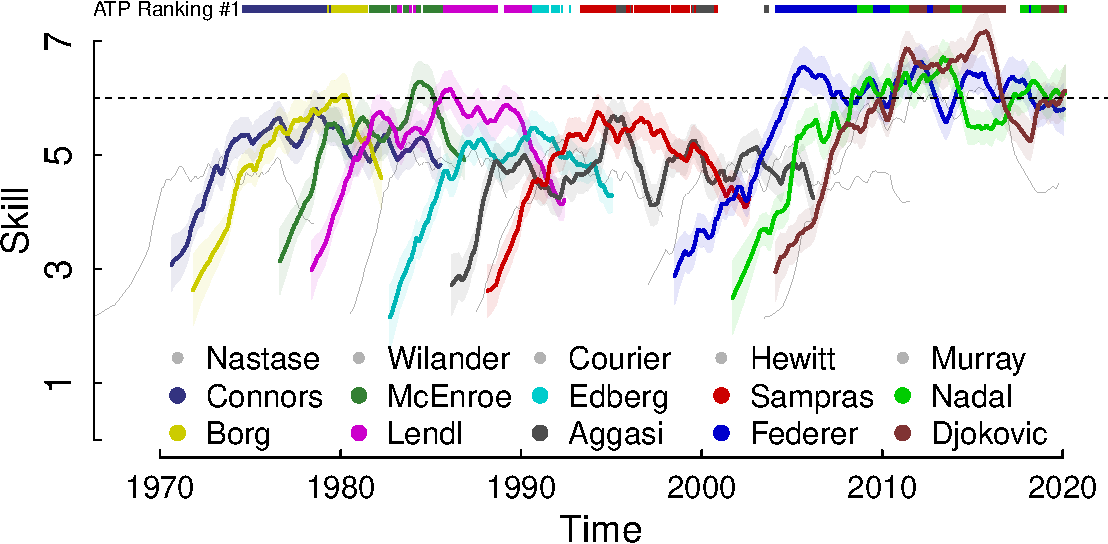
\includegraphics[width=.9\linewidth]{static/atp}
\end{subfigure}
\end{figure}



\columnbreak


























\centering

\texttt{github.com/glandfried/transitions}

{\fontsize{60}{72}\selectfont \textbf{Evolutionary - Probabilistic isomorphism} \\[0.2cm]
\LARGE \textbf{The irreversible emergence of cooperation and specialization} } \\[0.8cm]

\justify

\en{The current complexity of life is the consequence of a series of evolutionary transitions in which entities capable of self-replication after the transition become part of higher level cooperative units (eukaryotic cells, multicellular organisms, social systems). }%~\cite{maynardSmith1995-majorTransitions, szathmary1995-evolutionaryTransitions, szathmary2015-evolutionaryTransitions}
\es{La complejidad actual de la vida es consecuencia de una serie de transiciones evolutivas en las que entidades capaces de autoreplicación luego de la transición pasan a formar parte de unidades cooperativas de nivel superior (células eucariotas, organismos multicelululares (células eucariotas, organismos multicelulares, sistemas sociales). }%~\cite{maynardSmith1995-majorTransitions, szathmary1995-evolutionaryTransitions, szathmary2015-evolutionaryTransitions}
%
\en{In this paper we show that the advantage in favor of cooperation and specialization is so common in the history of life because of the multiplicative nature of evolutionary and probabilistic selection processes. }%
\es{En este trabajo mostramos que la ventaja a favor de la cooperación y la especialización es tan común en la historia de la vida debido a la naturaleza multiplicativa de los procesos de selección evolutiva y probabilística. }%

\vspace{1cm}


\textbf{Introduc\en{tion}\es{ción}}
\en{The evolutionary growth of a lineage over time, $\omega(t)$, is governed by a sequence of survival and reproduction rates $f(\cdot)$ }%
\es{El crecimiento evolutivo de un linaje en el tiempo, $\omega(t)$, esta gobernado por una secuencias estocástica de tasas de supervivencia y reproducción $f(\cdot)$ }%
%
\begin{equation} \label{eq:modelo_exponencial}
\omega(T) = \prod_t^T f(\Aa_t) \approx g^T \ \ \text{ with } \ \ f(\Aa) =
\begin{cases}
 1.5 & \Aa = \text{ \en{Head}\es{Cara} } \\
 0.6 & \Aa = \text{ \en{Tail}\es{Sello} }
\end{cases}
\end{equation}
%
\en{According to the \emph{replicator dynamic} equation \cite{taylor1978-replicatorDynamic}, the proportion of a strategy $\Ee$ in the population given the environment $\vec{\Aa}$ is }%
\es{Según el modelo estándar de evolución, conocido como \emph{replicator dynamic} \cite{taylor1978-replicatorDynamic}, la proporción de una estrategia en la población es }%
% schuster1983-replicatorDynamics, hofbauer2003-evolutionaryGameDynamics
%
\begin{equation} \label{eq:replicator_dynamic}  \tag{Isomorphism}
\scalebox{0.95}{
\begin{split}
P(\Ee|\Aa_1 \dots \Aa_T) = \frac{P(\Ee|\Aa_1 \dots \Aa _{T-1}) f(\Ee,\Aa_T)}{\sum_s P(\Ee|\Aa_1 \dots \Aa_{T-1}) f(\Ee,\Aa_T)}
\end{split}
}
\end{equation}
%
\en{Which is the characteristic growth rate $g$? }%
\es{¿Cuál es la tasa de crecimiento característica $g$? }%

\vspace{0.3cm}

\begin{figure}[H]
    \centering
    \begin{subfigure}[b]{0.49\linewidth}
    \includegraphics[width=\linewidth]{figures/pdf/ergodicity_expectedValue.pdf}
    \caption*{Arithmetic: $1.5 \cdot \frac{1}{2} + 0.6 \cdot  \frac{1}{2} = 1.05$}
    \end{subfigure}
    \begin{subfigure}[b]{0.49\linewidth}
    \includegraphics[width=\linewidth]{figures/pdf/ergodicity_individual_trayectories.pdf}
    \caption*{Geometric: $(1.5 \cdot 0.6)^{1/2} \approx 0.95$}
    \end{subfigure}
\end{figure}

\textbf{Result\en{s}\es{ados}}

\en{Cooperation reduces fluctuations, which increases the growth rate. }%
\es{La cooperación reduce las fluctuaciones, lo que aumenta la tasa de crecimiento. }%
%
\en{Defection increases fluctuations, which reduces the growth rate. }%
\es{La desercion aumenta las fluctuaciones, lo que reduce la tasa de crecimiento. }%
%
\begin{figure}[H]
    \centering
    \begin{subfigure}[b]{0.5\linewidth}
    \includegraphics[width=\linewidth]{figures/pdf/ergodicity_desertion.pdf}
    \end{subfigure}
\end{figure}

\en{As soon as cooperation emerges, an advantage in favor of specialist strategies appears. }%
\es{Apenas surge la cooperación, aparece una ventaja a favor de las estrategias especialistas. }%

\begin{figure}[H]
    \centering
    \begin{subfigure}[b]{0.49\linewidth}
    \includegraphics[width=\linewidth]{figures/pdf/tasa-temporal-0.pdf}
    \end{subfigure}
    \begin{subfigure}[b]{0.49\linewidth}
    \includegraphics[width=\linewidth]{figures/pdf/tasa-temporal-2.pdf}
    \end{subfigure}
    \label{fig:tasa-temporal-2}
\end{figure}

\en{Since specialist strategies are individually poorly adapted to the environment, an irreversibility of the evolutionary transition is created. }%
\es{Como la estrategias especialistas están individualmente mal adaptadas al ambiente, se crea una irreversbilidad de la transiciones evolutivas. }%

\vspace{0.5cm}

\textbf{Conclution.} The advantage in favor of cooperation and specialization is due to the multiplicative nature of evolutionary and probabilistic selection processes.



\end{multicols}
{ \footnotesize
%\nocite{*} % Print all references regardless of whether they were cited in the poster or not
\bibliographystyle{auxiliar/biblio/plos2015} % Plain referencing style
\bibliography{auxiliar/biblio/biblio.bib} % Use the example bibliography file sample.bib
}
\end{document}
